\documentclass[a4paper, norsk, 12pt]{article}
%\documentclass{article} % was article, thought i'd try with report...
\usepackage{float}
%\usepackage{fullpage} % 1 inch margins
%\usepackage{harvard} % harvard reference style++
\usepackage[hidelinks]{hyperref} % do not remember entirely what this does
%%\usepackage{minted} % [LINUXONLY] list environment with code highlighting
\usepackage[utf8]{inputenc} %To get æøå
\usepackage[norsk]{babel} %Does it norway'ish
%\setcounter{chapter}{-1} %chapter numeration to start on 0
%\usepackage{titlesec} %To make chapter headings different
\usepackage[margin=2.5cm]{geometry}
%\usepackage{longtable} %Table that breakes pages
%\usepackage{tabularx} %Table that breakes lines
%\usepackage{ltablex} %Table that combines longtable and tubularx. (Use \begin{tabularx}
\usepackage{graphicx} %To insert image
\usepackage{parskip} %Removes indent and make space between the part sections, like \medskip.
\usepackage[labelformat=empty]{caption} %Removes "Figur 'nr'" in \caption on images.
%\usepackage{color, colortbl} %To use colors in tabulars




%Removes the indent:
%\setlength\parindent{0pt}

%Changing the paragraph title look:
\makeatletter
\renewcommand\paragraph{\@startsection{paragraph}{4}{\z@}%
  {-3.25ex\@plus -1ex \@minus -.2ex} %To get new line after title
  {1.5ex \@plus .2ex}%
  {\normalfont\large\bfseries}}
\makeatother

%\titleformat{\chapter}[hang]{\bf\huge}{\thechapter}{2pc}{} %To make chapters nice
\title{Oblig 1 \\ IMT3441 \\ Database- og applikasjonsdrift}
\author{Solveig Sørheim 090880 \\ Martin Kristian Mellum 100874}
\date{\today}


\begin{document}
\begin{figure}[h!]
 \centering
  
\includegraphics[width=0.5\textwidth]{Images/hig_logo.png}
 %\caption{Bare noko eg skribla på Paint..}
 \maketitle       % make title
\end{figure}
\pagebreak
%%\section{Abstract} % not sure if needed
%%This section is to be written when all else is done. 100-200 words summarizing.
\tableofcontents % make table of contents
\pagebreak	% and break the page, because pretty

\section{Ukesoppgaver Nr. 1 - 18. januar}
\subsection{Oppgave 5}
\begin{itemize}
\item Vi installerte screen ganske greitt ved å følge retningslinjene i forelesingsfoilerne.
\item Startet en skreen ved å skrive screen -S “Navnet på screenen”
\item Gikk inn i en eksisterende screenen ved å skrive screen -r “Navn på screenen”
\item Bli med i en screen sammen en andre ved å skrive screen -x “Navn på screenen”
\item Går ut av screenen ved å presse Ctrl+a og Ctrl+d
\item Vi slettet en screen ved å først gå inn i screen sesjonen, deretter trykke control+a, og så shift+punktum, og deretter i kommandolinjen skrive quit.
\end{itemize}

\subsection{Oppgave 7}
\begin{figure}[h!]
 \centering
  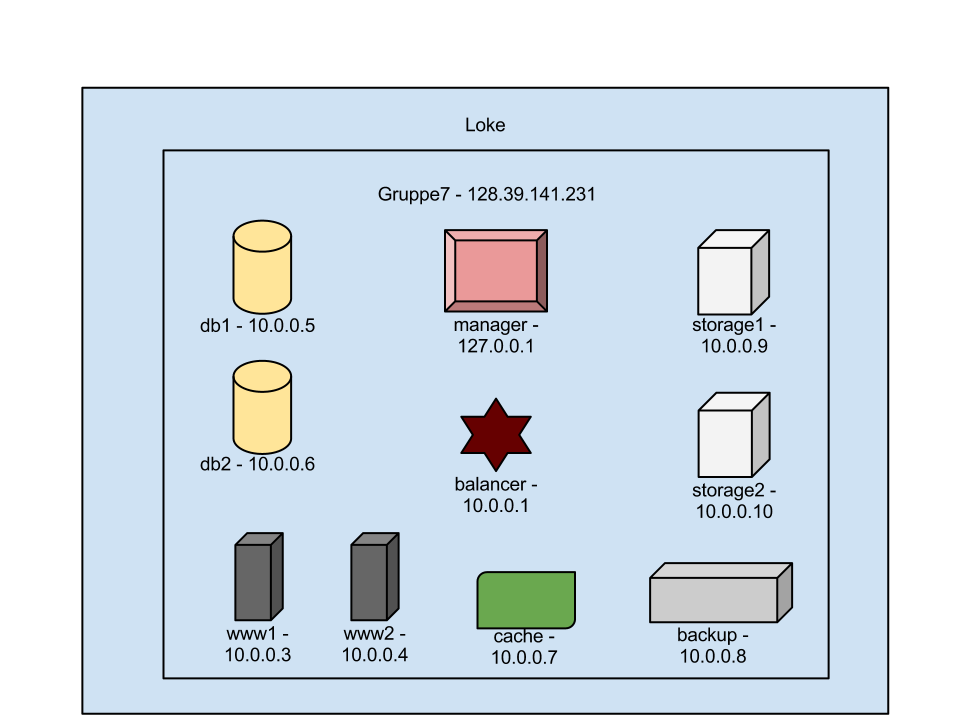
\includegraphics[width=1\textwidth]{Images/Gruppe7-IMT3441_Serverpark.png}
  \caption{Serverpark}
\end{figure}

\subsection{Oppgave 8}
\begin{description}
\item[10 \% Informasjonsintegritet - Backup \& Restore:]
 Systemadministrator må regelmessig ta backup av systemet, serverane og databasene. Dette kan gjøres automatisk, der systemadmin bare sjekker om backup vart gjort. Administratoren skal også ta større backuper ved andre tidspunkt. Dette tar ikke så lang tid. Å restore systemet skjer svært sjeldent.

\item[10 \% Adgangskontroll - Brukere \& Passord:]
Der kommer stadig nye brukere til systemet. Ettersom hvor mange brukere som kommer vil admin bruke variabelt med tid til dem. Men dette er en hurtig prosess, som ikke tar lang tid.

\item[35 \% Vedlikehold - Oppgradering \& Feilretting:]
Det viktigeste ansvaret til admin er vedlikehold, for å sørge for god vedlikehold vil minske risikoen for systemet. Der kommer stadig nye feil, og stadig må systemet oppgraderes. Derfor tar dette mest tid.

\item[25 \% Overvåking - Alarmer \& Ytelse over tid:]
Overvåkning er en veldig viktig del av jobben, og er måten man kan sjekke om alt annet fungerer slik det skal, men det tar tid og er en tidkrevende prossess å gå igjennom logger og system prosesser for å se at ting fortsetter å gå.

\item[10 \% Veiledning - Brukere \& Ny teknologi:]
Dette er en viktig del av jobben for at brukerene skal kunne bruke systemet, men det holder i stor grad å lage gode guider og FAQ’er, også slipper man mye manuell hjelping og spørsmål.

\item[10 \% Design - Infrastruktur:]
Design er en viktig jobb for å gjøre ting enkelt å bruke og forstå, men det gjøres gjerne en gang i starten, og i rykk og napp etterhvert som det må legges til ting, eller det gamle designet er utdatert, og er ikke noe som vanligvis endres å justeres hver dag.
\end{description}

\subsection{Oppgave 9}
Vi har fulgt forelesingsslidene når vi installerte munin. Da vi endret config-filen i manager så la vi inn de 9 andre servernavnene slik som eksempelet i forelesingsfoilene.
\begin{itemize}
\item Installert munin - done
\item Installert apache - done
\item Endret config filer - done
\end{itemize}

Installere noder og endret config:
\begin{itemize}
\item Storage1 - done
\item Storage2 - done
\item www1 - done
\item www2 - done
\item db1 - done
\item db2 - done
\item cache - done
\item manager - done
\item balancer -done
\item backup - done
\end{itemize}





%\chapter{Innledning}
\section{Introduksjon} 




%\clearpage
%\addcontentsline{toc}{section}{Referanser} %Add this section to content table
%\bibliographystyle{unsrt} % change for dcu, or something else entirely? unsrt is nice !- referanser
%\bibliography{Referanser}

%\addcontentsline{toc}{section}{Vedlegg} %Add this section to content table
%\section*{Vedlegg}

\end{document}